\section{Basics of Bayesian statistics}

\begin{figure}[h]
    \centering
    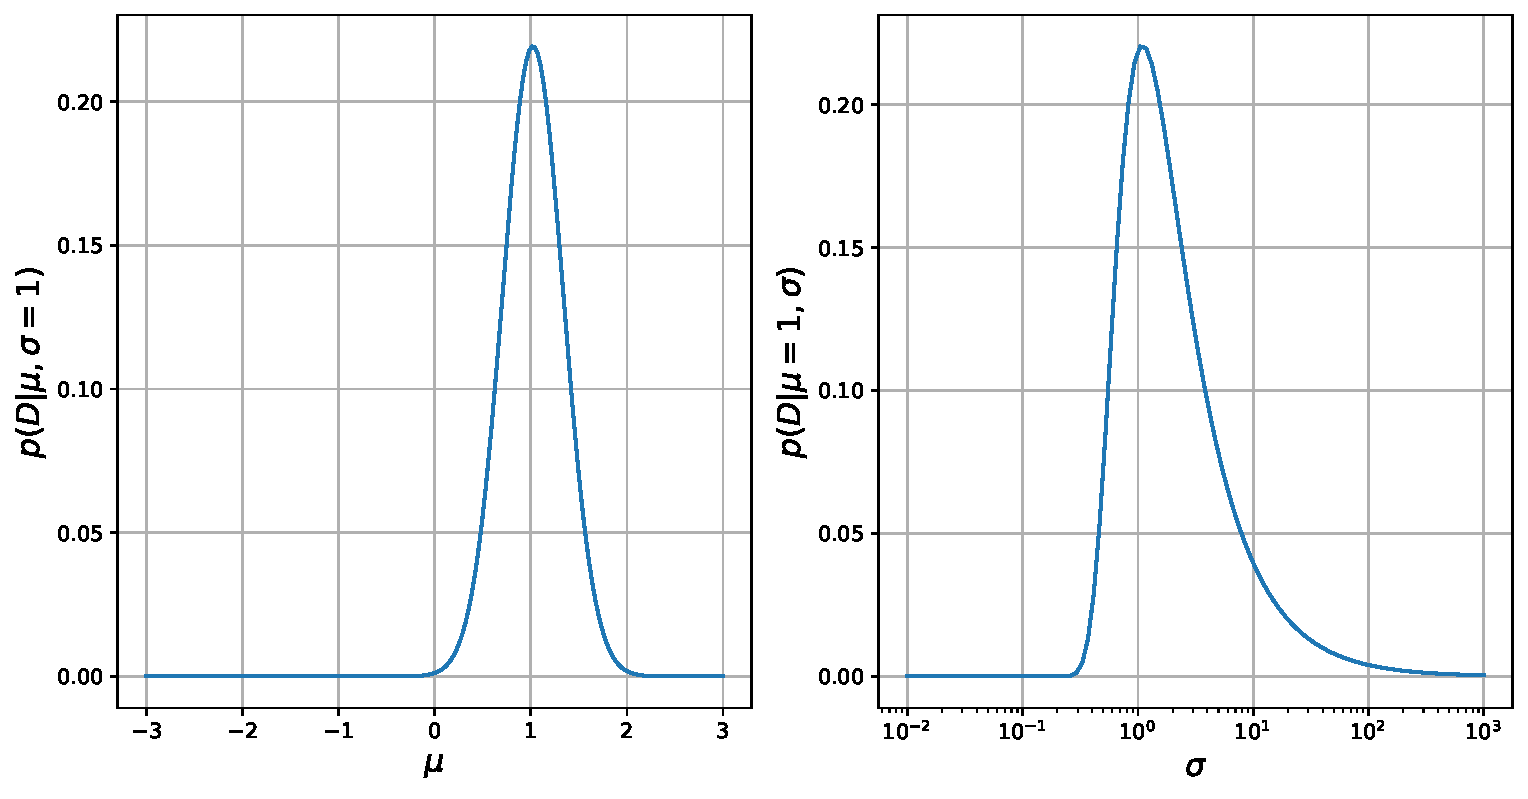
\includegraphics[width=0.9\linewidth]{pics/likelihood.pdf}
    \caption{Likelihood of the dataset $\mathcal{D}$ of $10$ samples from $\Normal(x\cond \mu = 1, \sigma^2 = 0.5^2)$.}
    \label{fig:likelihood}
\end{figure}

Maximum likelihood gives us a point-estimate of the parameters of our probabilistic model, and if the model is correct \kir{no} then we know that with the number of data points our estimate converges to the ground true value.
However, what if we plot the likelihood for other values of parameters?
In \cref{fig:likelihood}, we see that the likelihood function depending on the parameter also looks like some density, i.e. it is a positive function that vanishes at the infinity so it might be normalizable.

Indeed, consider the likelihood of some dataset $\mathcal{D}$, that corresponds to the normal model $p(x\cond \theta) = \Normal(x\cond \mu, \sigma^2)$. 
For the likelihood w.r.t $\mu$ (and some fixed $\sigma$) it's very straightforward
\begin{align}
    p(\mathcal{D}\cond \mu, \sigma=1) =~& \frac{1}{\sqrt{2\pi}}\exp\left(-\frac{1}{2}\sum_{i=1}^N(x_i-\mu)^2\right) = \frac{1}{\sqrt{2\pi}}\exp\left(-\frac{1}{2}\left(\sum_ix_i^2-2\mu\sum_i x_i + N\mu^2\right)\right)\\
    =~&\frac{1}{\sqrt{2\pi}}\exp\left(-\frac{\sqrt{N}^2}{2}\left(\mu^2-2\mu\hat{\mu} + \hat{\mu}^2 - \hat{\mu}^2 + \frac{1}{N}\sum_i x_i^2\right) \right)\\
    =~&\frac{1}{\sqrt{2\pi}}\exp\left(-\frac{1}{2(1/\sqrt{N})^2}\left(\mu-\hat{\mu}\right)^2 - \hat{\mu}^2 + \frac{1}{N}\sum_i x_i^2\right)\propto\Normal\left(\mu\cond \hat{\mu},\frac{1}{N}\right)\,,
    \label{eq:normal_likelihood}
\end{align}
where $\hat{\mu} = \frac{1}{N}\sum_i x_i$.
Thus, we see that the likelihood is proportional to the normal distribution w.r.t. $\mu$. 
However, it is the normal distribution w.r.t $\mu$ because it doesn't normalize to $1$. \kir{in some cases the function can be not normalizable in principle}

For the likelihood w.r.t. $\sigma$ (and fixed $\mu$), we have
\begin{align}
    p(\mathcal{D}\cond \mu=0, \sigma) =~& \frac{1}{\sqrt{2\pi\sigma^2}}\exp\left(-\frac{1}{2\sigma^2}\sum_{i=1}^Nx_i^2\right) \propto \left(\frac{1}{\sigma^2}\right)^{N/2}\exp\left(-\left(\frac{1}{2}\sum_{i=1}^Nx_i^2\right)\frac{1}{\sigma^2}\right)\\
    =~& \gamma^{N/2}\exp\left(-\left(\frac{1}{2}\sum_{i=1}^Nx_i^2\right)\gamma\right) \propto \mathcal{G}\left(\gamma\cond N/2+1, \frac{1}{2}\sum_{i=1}^Nx_i^2\right)\,,
\end{align}
where we introduced the parameter $\gamma = 1/\sigma^2$.
The likelihood function is proportional to the density of the gamma distribution (see below), but it's not the gamma distribution because it doesn't normalize to $1$.

\begin{definition}[Gamma distribution]\label{def:gamma_pdf}
    Consider the density proportional to 
    \begin{align}
        \mathcal{G}(x\cond a,b) = \frac{b^a}{\Gamma(a)}x^{a-1}\exp(-b x)\,,
    \end{align}
    where $\Gamma(\cdot)$ is the gamma function.
\end{definition}

To sum up, we see that the likelihood already defines something like a distribution on the set of parameters.
Thus, we should consider treating parameters as random variables!

\subsection{Bayesian reasoning}

When treating parameters as random variables, let's start with the likelihood model, i.e. let's assume that the following holds
\begin{align}
    p(\mathcal{D} \cond \theta) = \prod_i p(x_i\cond \theta)\,,
\end{align}
and the model $p(x\cond \theta)$ is given.
Remember that the entire information about $x$ and $\theta$ is in their joint distribution, whose density we can write down as follows (using \cref{def:cond_dist})
\begin{align}
    \underbrace{p(x,\theta)}_{\text{joint}} = \underbrace{p(x\cond \theta)}_{\text{likelihood}}\underbrace{p(\theta)}_{\text{prior}}\,.
\end{align}
Thus, if we know or introduce the prior distribution $p(\theta)$, we know everything about the random variables $x$ and $\theta$.

Namely, using the definition of the conditional distribution (or \cref{th:bayes}), we can write down the following
\begin{align}
\label{eq:posterior_density}
    p(\theta \cond \mathcal{D}) = \frac{p(\mathcal{D} \cond \theta)p(\theta)}{p(\mathcal{D})} = \frac{p(\mathcal{D} \cond \theta)p(\theta)}{\int d\theta\; p(\mathcal{D} \cond \theta)p(\theta)}\,.
\end{align}
\begin{mybox}
\begin{definition}[Posterior Distribution]\label{def:posterior}
    Distribution corresponding to the density $p(\theta \cond \mathcal{D})$ from \cref{eq:posterior_density} is called the posterior distribution.
\end{definition}
\end{mybox}

Let's try choosing prior $p(\theta)$ such that we know the posterior distribution $p(\theta\cond \mathcal{D})$ immediately.

\begin{example}
    For the likelihood, consider the normal distribution with the parameter $\mu$ and fixed $\sigma$
    \begin{align}
        p(x\cond \theta) = \Normal(x\cond \mu,\sigma^2=1)\,.
    \end{align}
    From \cref{eq:normal_likelihood}, we already have
    \begin{align}
        p(\mathcal{D}\cond \mu, \sigma=1)\propto\Normal\left(\mu\cond \hat{\mu},\frac{1}{N}\right) \propto \exp\left(-\frac{1}{2(1/\sqrt{N})^2}(\mu-\hat{\mu})^2\right)\,,
    \end{align}
    where $\hat{\mu} = \frac{1}{N}\sum_i x_i$.
    The posterior distribution is defined as
    \begin{align}
        p(\mu \cond \mathcal{D}) \propto \exp\left(-\frac{1}{2(1/\sqrt{N})^2}(\mu-\hat{\mu})^2\right)p(\mu)\,.
    \end{align}
    Let's choose the prior distribution $p(\mu)$ so that the functional form of the posterior distribution is the same as of the prior distribution.
    That is, consider $p(\mu) = \Normal(\mu\cond m,s^2)$
    \begin{align}
        p(\mu \cond \mathcal{D}) \propto~& \exp\left[-\frac{1}{2(1/\sqrt{N})^2}(\mu-\hat{\mu})^2-\frac{1}{2s^2}(\mu-m)^2\right] \propto \exp\left[-\frac{1}{2}\left(\left(N+\frac{1}{s^2}\right)\mu^2 -2\mu\left(N\hat{\mu}+\frac{m}{s^2}\right)\right)\right] \\
        =~& \exp\left[-\frac{1}{2}\left(\frac{Ns^2+1}{s^2}\right)\left(\mu^2 -2\mu\left(\frac{Ns^2\hat{\mu}+m}{Ns^2+1}\right)\right)\right] \\
        \propto~& \exp\left[-\frac{1}{2}\left(\frac{Ns^2+1}{s^2}\right)\left(\mu -\left(\frac{Ns^2\hat{\mu}+m}{Ns^2+1}\right)\right)^2\right] = \Normal\left(\mu\cond \frac{Ns^2\hat{\mu}+m}{Ns^2+1}, \frac{s^2}{Ns^2+1}\right)
    \end{align}
\end{example}
Note that
\begin{align}
    \lim_{N\to\infty} \frac{Ns^2\hat{\mu}+m}{Ns^2+1} = \lim_{N\to\infty}\hat{\mu} = \lim_{N\to\infty}\mu_{\text{MLE}}\,,
\end{align}
and for large $N$, we have
\begin{align}
    \frac{s^2}{Ns^2+1} \approx \frac{1}{N}\,,
\end{align}
as we had before for the likelihood w.r.t. $\sigma$.

By finding the prior such that the posterior is easy to find we have motivated the following definition.
\begin{mybox}
\begin{definition}[Conjugate distribution]\label{def:conjugate_dist}
    For the likelihood $p(x\cond \theta)$, if the parametric family of the posterior $p(\theta\cond x)$ is the same as the parametric family of the prior $p(\theta)$ these distributions are called conjugate.
    Oftentimes, people just say conjugate prior $p(\theta)$ to the likelihood $p(x\cond \theta)$.
\end{definition}
\end{mybox}

\begin{example}
    For the likelihood, consider the normal distribution with the parameter $\sigma$ and fixed $\mu$
    \begin{align}
        p(x\cond \theta) = \Normal(x\cond \mu=0,\sigma^2)\,.
    \end{align}
    From before, we have
    \begin{align}
    p(\mathcal{D}\cond \mu=0, \sigma) \propto \mathcal{G}\left(\gamma\cond N/2+1, \frac{1}{2}\sum_{i=1}^Nx_i^2\right)\,,
    \end{align}
    The posterior distribution is defined as
    \begin{align}
        p(\gamma \cond \mathcal{D}) \propto \gamma^{N/2}\exp\left(-\left(\frac{1}{2}\sum_{i=1}^Nx_i^2\right)\gamma\right)p(\gamma)\,.
    \end{align}
    Let's choose the prior distribution $p(\gamma)$ so that the functional form of the posterior distribution is the same as of the prior distribution.
    That is, consider $p(\gamma) = \mathcal{G}(\gamma\cond a,b)$
    \begin{align}
        p(\gamma \cond \mathcal{D}) \propto \gamma^{N/2}\exp\left(-\left(\frac{1}{2}\sum_{i=1}^Nx_i^2\right)\gamma\right)\gamma^{a-1}\exp(-b\gamma) \propto \mathcal{G}\left(\gamma\cond N/2+a, b+\frac{1}{2}\sum_{i=1}^Nx_i^2\right)\,.
    \end{align}
\end{example}

\begin{exercise}
    Consider $x_1,\ldots,x_N$ --- iid samples from the exponential density function
    \begin{align}
        p(x\cond \lambda) = \lambda\exp(-\lambda x)\,, \;\; x \geq 0\,, \lambda > 0.
    \end{align}
    Find the conjugate prior $p(\lambda)$ and the corresponding posterior $p(\lambda\cond \mathcal{D})$.
\end{exercise}

\begin{exercise}
    Consider $x_1,\ldots,x_N$ --- iid samples from the Poisson distribution $\text{Poiss}(\lambda)$
    \begin{align}
        P(X = k\cond \lambda) = \exp(-\lambda)\frac{\lambda^k}{k!}.
    \end{align}
    Find the conjugate prior $p(\lambda)$ and the corresponding posterior $p(\lambda\cond \mathcal{D})$.
\end{exercise}

\begin{exercise}
    Consider $x_1,\ldots,x_N$ --- iid samples from the Bernoulli distribution $\text{Bernoulli}(\theta)$
    \begin{align}
        p(x\cond \theta) = \theta^x(1-\theta)^{(1-x)}.
    \end{align}
    Find the conjugate prior $p(\theta)$ and the corresponding posterior $p(\theta\cond \mathcal{D})$. Does it matter if instead we consider one sample from the Binomial with probability of success $\theta$ and number of trials $N$?
\end{exercise}

\kir{I'll just put this here}
\begin{mybox}
\begin{definition}[Beta distribution]\label{def:beta_density}
    Consider the density proportional to 
    \begin{align}
        \mathcal{B}(x\cond a,b) = \frac{\Gamma(a+b)}{\Gamma(a)\Gamma(b)}x^{a-1}(1-x)^{b-1} = \frac{1}{B(a,b)}x^{a-1}(1-x)^{b-1}\,,
    \end{align}
    where $\Gamma(\cdot)$ and $B(\cdot)$ are the gamma and beta functions correspondingly.
\end{definition}
\end{mybox}

When it's hard to find the entire posterior distribution, one can use its mode, which is easier to find.
\begin{mybox}
\begin{definition}[Maximum A posteriori (MAP)]\label{def:map}
    The mode of the posterior distribution is called the Maximum A posteriori (MAP) estimate and is defined as follows
    \begin{align}
        \theta_{\text{MAP}} = \argmax_{\theta \in \Theta} p(\theta \cond \mathcal{D}) = \argmax_{\theta \in \Theta} \frac{p(\mathcal{D} \cond \theta)p(\theta)}{p(\mathcal{D})} = \argmax_{\theta \in \Theta} p(\mathcal{D} \cond \theta)p(\theta)\,.
    \end{align}
\end{definition}
\end{mybox}

Finally, to make new prediction, one can take into account all the possible parameters from the posterior distribution.
Namely, let's say we want to get the distribution of observations $x$ after observing the dataset $\mathcal{D}$, then we can write \kir{absolutely mindless mathematical tautology}
\begin{align}
    p(x\cond \mathcal{D}) = \int d\theta\; p(x,\theta \cond \mathcal{D}) = \int d\theta\; p(x \cond \theta, \mathcal{D}) p(\theta \cond \mathcal{D})\,,
\end{align}
after we assume that all the information about the dataset is in our parameters $\theta$.
In other words, having the parameters $\theta$ is all we need for making the probabilistic model, i.e. $p(x \cond \theta, \mathcal{D}) = p(x \cond \theta)$.
Under this strong assumption, we proceed as
\begin{align}
    p(x\cond \mathcal{D}) = \int d\theta\; p(x \cond \theta) p(\theta \cond \mathcal{D}) = \mean_{p(\theta \cond \mathcal{D})} p(x \cond \theta)\,,
\end{align}
i.e. the probabilistic model of $x$, after observing the dataset $\mathcal{D}$ is defined as an average of probabilities/densities over all possible values of parameters sampled from the posterior distribution.
\begin{mybox}
\begin{definition}[Predictive Distribution]\label{def:predictive_dist}
    Given the likelihood $p(x \cond \theta)$ and the posterior $p(\theta \cond \mathcal{D})$, one defines the predictive distribution as follows
    \begin{align}
        p(x\cond \mathcal{D}) = \int d\theta\; p(x \cond \theta) p(\theta \cond \mathcal{D}) = \mean_{p(\theta \cond \mathcal{D})} p(x \cond \theta)\,.
    \end{align}
\end{definition}
\end{mybox}

\subsection{Exponential family}

There is a large and important family of distributions that allows for the Bayesian inference.
\begin{mybox}
\begin{definition}[Exponential family]\label{def:expo_family}
    The exponential family of random variables is all random variables which density has the following functional form
    \begin{align}
        p(x\cond \theta) = \frac{f(x)}{g(\theta)}\exp\left(\theta^Tu(x)\right)\,.
    \end{align}
\end{definition}
\end{mybox}

First, let's play around with the definition.
For instance, let's see what we can get from the normalization of the density.
\begin{align}
    \int dx\; p(x\cond \theta) =~& \int dx\; \frac{f(x)}{g(\theta)}\exp\left(\theta^Tu(x)\right) = 1\,,\\
    g(\theta) =~& \int dx\; f(x)\exp\left(\theta^Tu(x)\right)\,.
\end{align}
It is reasonable to call $g(\theta)$ a normalization constant of this distribution.
Note that the derivative of the normalization constant has interesting properties
\begin{align}
    \deriv{}{\theta_i}g(\theta) =~& \int dx\; f(x)\deriv{}{\theta_i}\exp\left(\theta^Tu(x)\right) = \int dx\; f(x)\exp\left(\theta^Tu(x)\right)u_i(x) = g(\theta)\int dx\; p(x\cond \theta) u_i(x)\,,\\
    \deriv{}{\theta_i}\log g(\theta) =~& g(\theta)\int dx\; p(x\cond \theta) u_i(x) = \mean_{p(x\cond \theta)}u_i(x)\,.
\end{align}
Thus, we have
\begin{proposition}
\label{prop:grad_norm_constant}
    For the density $p(x\cond \theta)$ from the exponential family, we have
    \begin{align}
        \nabla_\theta\log g(\theta) = \mean_{p(x\cond \theta)}u(x)\,.
    \end{align}
\end{proposition}

\begin{exercise}
For the exponential family $p(x\cond \theta) = \frac{f(x)}{g(\theta)}\exp\left(\theta^Tu(x)\right)$, find the expression for
\begin{align}
    \deriv{^2}{\theta_i\theta_j}\log g(\theta) = ?
\end{align}
\end{exercise}

Let's find the maximum likelihood estimator for this family
\begin{align}
    \log p(\mathcal{D}\cond \theta) =~& \sum_{i=1}^N \left[\log f(x_i) - \log g(\theta) + \theta^Tu(x_i)\right]\,,\\
    \nabla_\theta\log p(\mathcal{D}\cond \theta) =~& \sum_{i=1}^N \left[ - \nabla_\theta\log g(\theta) + u(x_i)\right] = 0\,,\\
    \nabla_\theta\log g(\theta) =~& \frac{1}{N}\sum_{i=1}^Nu(x_i)\,.
\end{align}
Using \cref{prop:grad_norm_constant}, we have that, for $\theta_{\text{MLE}}$, the expectation of statistics $u(x)$ equals empirical expectation of statistics $u(x)$ on the observed data, i.e.
\begin{align}
    \mean_{p(x\cond \theta_{\text{MLE}})}u(x) = \frac{1}{N}\sum_{i=1}^Nu(x_i)\,.
\end{align}
Note we need only values of $u(x_i)$ on our data to completely determine the maximum likelihood estimation of our parameters $\theta$. This motivates the following definition
\begin{mybox}
\begin{definition}[Sufficient statistics]\label{def:suff_stats}
When the density $p(x\cond \theta)$ can be factorized as
\begin{align}
    p(x\cond \theta) = p_1(x)p_2(u(x),\theta)\,,
\end{align}
the function $u(x)$ is called sufficient statistics.
\end{definition}
\end{mybox}

\begin{example}
Consider the normal density
\begin{align}
    \Normal(x\cond \mu, \sigma^2) = \frac{1}{\sqrt{2\pi\sigma^2}}\exp\left(-\frac{1}{2\sigma^2}(x-\mu)^2\right) = \frac{1}{\sqrt{2\pi\sigma^2}}\exp\left(-\frac{x^2}{2\sigma^2} + \frac{x\mu}{\sigma^2} -\frac{\mu^2}{2\sigma^2}\right)\,.
\end{align}
From the definition of exponential family, we can write
\begin{align}
    u(x) = \begin{bmatrix}
        x\\
        x^2
    \end{bmatrix}\,,\;\;
    \theta = \begin{bmatrix}
        \frac{\mu}{\sigma^2}\\
        -\frac{1}{2\sigma^2}
    \end{bmatrix}\,,\;\;
    g(\theta)^{-1} = \frac{1}{\sqrt{2\pi\sigma^2}}\exp\left(-\frac{\mu^2}{2\sigma^2}\right) = \sqrt{\frac{-\theta_2}{\pi}}\exp\left(\frac{\theta_1^2}{4\theta_2}\right)\,.
\end{align}
Thus, we have a different parameterization of the normal distribution. Let's find the expectation from this parametric form.
\begin{align}
    \deriv{}{\theta_1}\log g(\theta) =~& -\frac{\theta_1}{2\theta_2} = \mu\,,\\
    \deriv{}{\theta_2}\log g(\theta) =~& -\frac{1}{2\theta_2}+\frac{\theta_1^2}{4\theta_2^2} = \sigma^2 + \mu^2\,.
\end{align}
Hence, we see that we can find expectations of sufficient statistics without integration \kir{integration is principally much harder than differentiation}
\end{example}
When we write down some density in the form of \cref{def:expo_family}, the parameters $\theta$ are called \textit{natural parameters}.

Let's find the conjugate distributions to the exponential family
\begin{align}
    p(\theta\cond \mathcal{D}) \propto~& \prod_i p(x_i\cond \theta)p(\theta) = \left[\prod_i\frac{f(x_i)}{g(\theta)}\right]\exp\left(\sum_i\theta^Tu(x_i)\right)p(\theta)\\
    =~& \left[\prod_i f(x_i)\right]\exp\left(\sum_i\theta^Tu(x_i)\right)\frac{p(\theta)}{g(\theta)^N}\,.
\end{align}
Based on this form, we can choose the prior
\begin{align}
    p(\theta\cond \eta,\nu) = \frac{1}{h(\eta,\nu)}\frac{1}{g(\theta)^\nu}\exp\left(\theta^T\eta\right)\,.
\end{align}
Then
\begin{align}
    p(\theta\cond \mathcal{D}) \propto~& \frac{1}{g(\theta)^N}\exp\left(\sum_i\theta^Tu(x_i)\right)\frac{1}{h(\eta,\nu)}\frac{1}{g(\theta)^\nu}\exp\left(\theta^T\eta\right) \propto \frac{1}{g(\theta)^{\nu+N}}\exp\left(\theta^T\left(\eta +\sum_iu(x_i)\right)\right)\\
    p(\theta\cond \mathcal{D}) \propto~& p(\theta\cond \eta +\sum_iu(x_i),\nu + N)\,.
\end{align}

\begin{exercise}
    Represent the gamma distribution
    \begin{align}
        \mathcal{G}(x\cond a,b) = \frac{b^a}{\Gamma(a)}x^{a-1}\exp(-b x)\,,
    \end{align}
    as a density from the exponential family, find the expectations of the sufficient statistics.
\end{exercise}

\begin{exercise}
    Represent the beta distribution
    \begin{align}
        \mathcal{B}(x\cond a,b) = \frac{\Gamma(a+b)}{\Gamma(a)\Gamma(b)}x^{a-1}(1-x)^{b-1} = \frac{1}{B(a,b)}x^{a-1}(1-x)^{b-1}\,,
    \end{align}
    as a density from the exponential family, find the expectations of the sufficient statistics.
\end{exercise}

\subsection{Maximum Entropy Principle \citep{jaynes1957information}}

Consider a distribution over a finite set of outcomes $\{1,\ldots,M\}$ with probabilities $\{p_1,\ldots,p_M\}$. 
Clearly, when $p_1 = 1$ and $p_i = 0\,, i = 2,\ldots, M$ the distribution becomes degenerate and we can say for sure that all the outcomes are going to be $1$.
This motivates the following question: can we introduce some function $\ent(\{p_1,\ldots,p_M\})$ that measures the `uncertainty' of the given distribution.
To answer these question let's start with the following three axioms:
\begin{enumerate}
    \item The function $\ent(\{p_1,\ldots,p_M\})$ has to be continuous w.r.t. $p_i$. \kir{indeed, we don't expect any discontinuous transitions}
    \item For $p_1 = \ldots = p_M = 1/M$, the function has to be increasing w.r.t. $M$. \kir{that means that more outcomes introduce more uncertainty}
    \item The function $\ent(\{p_1,\ldots,p_M\})$ has to be invariant over the different outcomes in the sigma algebra \kir{there are multiple ways to compute the uncertainty of the same distribution by grouping the events in different groups. uncertainty has to be invariant w.r.t. all these ways.}. Indeed, consider $K$ disjoint sets of outcomes (see \cref{fig:composability_H}) where the total probability of events in the set $k$ is $\hat{p}_k$. The outcomes $\{x_{k1},\ldots,x_{kM_k}\}$ within the set $k$ define new distribution with probabilities $\{p_{k1}/\hat{p}_k,\ldots,p_{kM_k}/\hat{p}_k\}$.
    The distribution over the sets is $\{\hat{p}_1,\ldots,\hat{p}_K\}$.
    Thus, the uncertainty over the original events $\{1,\ldots,M\}$ is can be evaluated as the uncertainty over $\{\hat{p}_1,\ldots,\hat{p}_K\}$ and then the expectation over uncertainties within every subgroup, i.e.
    \begin{align}
        \ent(\{\hat{p}_1,\ldots,\hat{p}_K\}) + \sum_{k=1}^K \hat{p}_k\ent(\{p_{k1}/\hat{p}_k,\ldots,p_{kM_k}/\hat{p}_k\}) = \ent(\{p_1,\ldots,p_M\})\,.
    \end{align}
\end{enumerate}

\begin{figure}
    \centering
    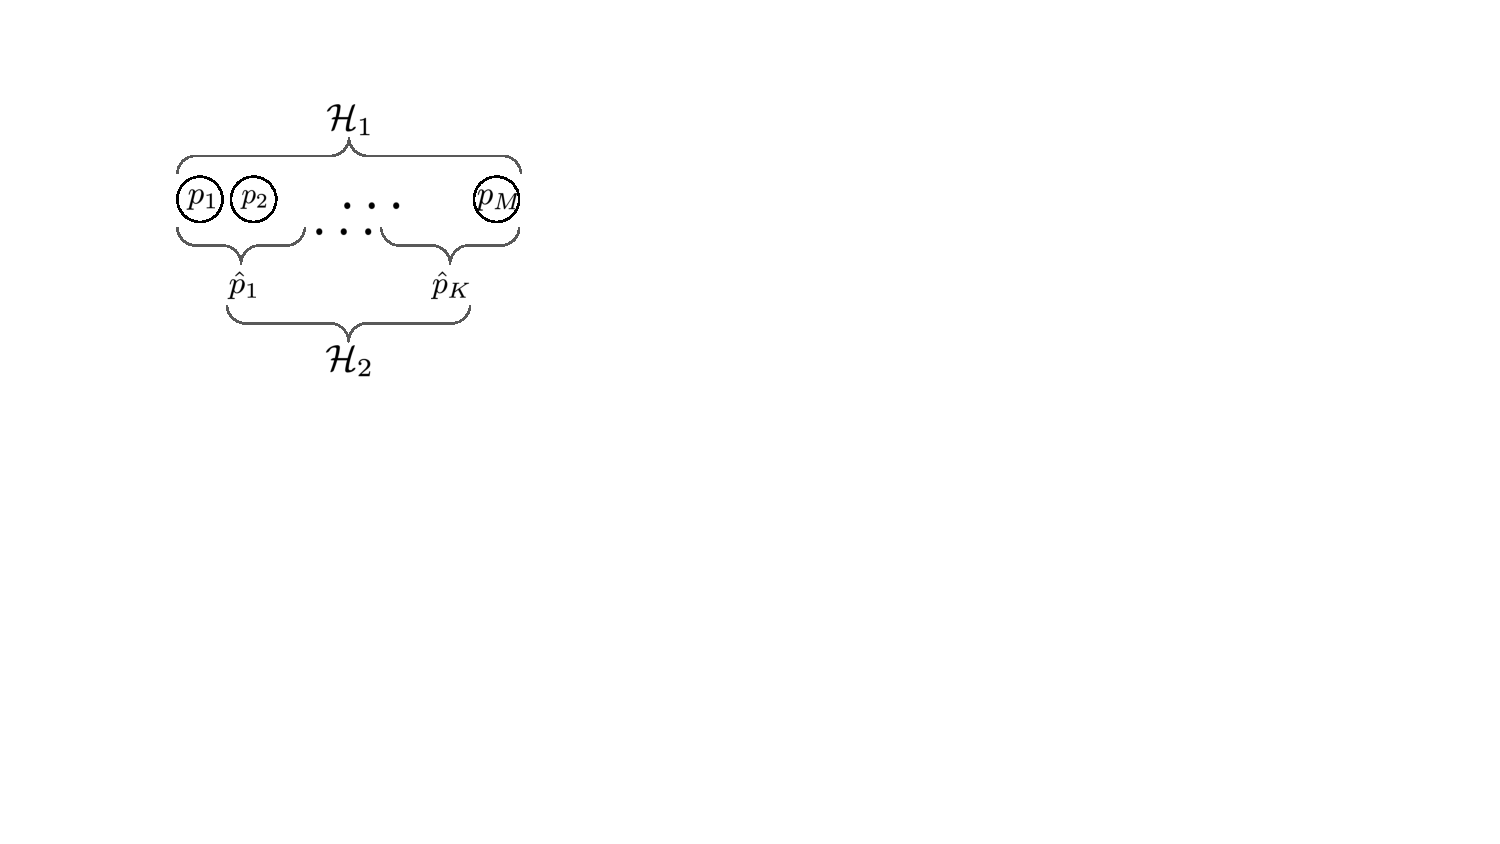
\includegraphics[width=0.3\linewidth]{pics/composability_H.pdf}
    \caption{Invariance of the entropy w.r.t. grouping events into disjoint sets.}
    \label{fig:composability_H}
\end{figure}

Let's consider a distribution $\{p_1,\ldots,p_M\}$, where the probabilities are given as rational numbers
\begin{align}
    p_i = \frac{m_i}{\sum_{j=1}^M m_j}\,.
\end{align}
Let's `ungroup' every event $x_i$ into $m_i$ events with uniform probabilities and use the invariance axiom
\begin{align}
    \ent(\{p_1,\ldots,p_M\}) + \sum_{i=1}^M p_i\ent(\{1/m_i,\ldots,1/m_i\}) = \ent(\{1/\sum_{i=1}^M m_i,\ldots,1/\sum_{i=1}^M m_i\})\,.
    \label{eq:rational_groups}
\end{align}
It's useful to introduce the following function
\begin{align}
    A(M) \coloneqq \ent(\{1/M,\ldots,1/M\})\,,
\end{align}
and note that, for $m_i = m\,,\;\forall i$, \cref{eq:rational_groups} becomes
\begin{align}
    A(M) + \sum_{i=1}^M \frac{m}{mM} A(m) = A(mM)\\
    A(M) + A(m) = A(mM)\,.
\end{align}
Clearly, for $m=1$,
\begin{align}
    A(M) + A(1) = A(M) \implies A(1) = 0\,.
\end{align}
For $m=M$,
\begin{align}
    A(m) + A(m) = A(m^2) \implies nA(m) = A(m^n)\,.
\end{align}
Thus, we see that $A(m) = \log m$ and using \cref{eq:rational_groups}, we have
\begin{align}
    \ent(\{p_1,\ldots,p_M\}) = - \sum_{i=1}^M p_i\log n_i + \log \sum_{j=1}^M \log n_j\, = - \sum_{i=1}^M p_i\log p_i\,.
\end{align}
This motivates the following definition.

\begin{mybox}
\begin{definition}[Entropy]\label{def:entropy}
    For a distribution over discrete outcomes $\{1,\ldots,M\}$ with probabilities $\{p_1,\ldots,p_M\}$, entropy is defined as
    \begin{align}
        \ent(\{p_1,\ldots,p_M\}) = -\sum_{i=1}^M p_i \log p_i\,.
    \end{align}
\end{definition}
\end{mybox}

Once we introduce the measure of uncertainty, or the measure of information, we can start asking questions about the distributions with the most uncertainty or the least information.
For example, consider a dataset $\mathcal{D}$ of observations $\{x_i\}_{i=1}^N$, and the statistics $u_k(x)$ evaluated on it, i.e.
\begin{align}
    \mean_{x\sim \mathcal{D}} u_k(x) = \frac{1}{N}\sum_{i=1}^N u_k(x_i) = \mu_k\,, \;\; k = 1,\ldots,K\,.
\end{align}
Then we can look for \textit{the distribution that explains the data and doesn't explain anything else}, as defined in the following definition.

\begin{mybox}
\begin{definition}[Maximum entropy principle]\label{def:max_ent}
    For the dataset $\mathcal{D}$ with statistics $\mu_k$, the maximum entropy principle defines the distribution as a solution to the following optimization problem
    \begin{align}
        \max_{p} \ent(\{p_1,\ldots,p_M\})\,, \;\; \text{ s.t. }\;\; \sum_{i=1}^M p_i u_k(i) = \mu_k\,, k = 1,\ldots,K\,.
    \end{align}
\end{definition}
\end{mybox}
Let's find the solution of this optimization problem.
First, the Lagrangian corresponding to the constrained optimization problem is
\begin{align}
    \mathcal{L}(\lambda, p) =~& \ent(\{p_1,\ldots,p_M\}) + \sum_{k=1}^K\lambda_k\left(\sum_{i=1}^M p_i u_k(i) - \mu_k\right) \\
    =~& -\sum_{i=1}^M p_i \log p_i + \sum_{k=1}^K\lambda_k\left(\sum_{i=1}^M p_i u_k(i) - \mu_k\right)\,.
\end{align}
We have to solve
\begin{align}
    \min_\lambda \max_p \mathcal{L}(\lambda, p)\,.
\end{align}
Taking the derivative w.r.t. $p$, we have
\begin{align}
    \deriv{\mathcal{L}}{p_j} = -\log p_j - 1 + \sum_k \lambda_k u_k(j) = 0 \implies p_j \propto \exp\left(\sum_k \lambda_k u_k(j)\right)\,,\\
    p_j = \frac{1}{Z_\lambda} \exp\left(\sum_k \lambda_k u_k(j)\right)\,, \;\; Z_\lambda = \sum_{j}^{M} \exp\left(\sum_k \lambda_k u_k(j)\right)\,.
\end{align}
Thus, we have
\begin{align}
    \min_\lambda \max_p \mathcal{L}(\lambda, p) =~& \min_\lambda \log Z_\lambda - \sum_{i=1}^M p_i \sum_k \lambda_k u_k(i) + \sum_{k=1}^K\lambda_k\left(\sum_{i=1}^M p_i u_k(i) - \mu_k\right)\\
    =~& \min_\lambda -\mean_{x\sim \mathcal{D}} \left[\sum_{k=1}^K \lambda_k u_k(x)-\log Z_\lambda\right] = \max_\lambda \mean_{x\sim \mathcal{D}} \log p_x\,,
\end{align}
which, as we see, is equivalent to maximum likelihood in the exponential family.

The same reasoning applies for the continuous random variables as follows.
\begin{mybox}
\begin{definition}[Differential Entropy]\label{def:diff_entropy}
    For a continuous random variable with the density $q(x)$, differential entropy is defined as
    \begin{align}
        \ent(q) = -\int dx\; q(x) \log q(x) = -\mean_{q(x)}\log q(x)\,.
    \end{align}
\end{definition}    
\end{mybox}
Let's see what the maximum entropy principle tells us for the differential entropy.
\begin{align}
    \max_{q} \ent(q(x))\,, \;\; \text{ s.t. }\;\; \int dx\; q(x)u_n(x) = \mu_n\,, n = 1,\ldots,N\,.
\end{align}
The Lagrangian corresponding to the problem is
\begin{align}
    \mathcal{L}(q,\lambda) =~& \ent(q) + \sum_{n=1}^N\lambda_n \left(\int dx\; q(x)u_n(x) - \mu_n\right) \\
    =~& -\int dx\;q(x)\log q(x) + \sum_{n=1}^N\lambda_n \left(\int dx\; q(x)u_n(x) - \mu_n\right)\,,
\end{align}
and the dual optimization problem is
\begin{align}
    \min_\lambda \max_q \mathcal{L}(q,\lambda)\,.
\end{align}
Let's write down the extremum condition for the inner optimization problem $\min_q \mathcal{L}(q,\lambda)$
\begin{align}
    \frac{\delta \mathcal{L}}{\delta q} = -\log q(x) + \sum_n\lambda_n u_n(x) = 0 \implies q(x) \propto \exp\left(\sum_n\lambda_n u_n(x)\right)\,.
\end{align}
From the normalization condition, we have
\begin{align}
    q(x\cond \lambda) = \frac{1}{Z_\lambda}\exp\left(\sum_n\lambda_n u_n(x)\right)\,,\;\; Z_\lambda = \int dx\; \exp\left(\sum_n\lambda_n u_n(x)\right)\,.
\end{align}
\begin{align}
    \mathcal{L}(q,\lambda) =~& \log Z_\lambda - \int dx\;q(x\cond \lambda)\left(\sum_n\lambda_n u_n(x)\right) + \sum_{n=1}^N\lambda_n \left(\int dx\; q(x\cond \lambda)u_n(x) - \mu_n\right) \\
    =~& \log Z_\lambda -\sum_{n=1}^N\lambda_n\mu_n = \log Z_\lambda -\sum_{n=1}^N\lambda_n\mean_{x \sim \mathcal{D}}\mu_n(x) = -\mean_{x \sim \mathcal{D}}\log q(x\cond \lambda)\,.
\end{align}
Thus, we have the following optimization problem
\begin{align}
    \min_\lambda \max_q \mathcal{L}(q,\lambda) = \min_\lambda - \log q(\mathcal{D}\cond \lambda) = \max_\lambda \log q(\mathcal{D}\cond \lambda)\,,
\end{align}
and we can make the following statement.

\begin{theorem}
    Maximum entropy principle corresponds to the maximum likelihood in the exponential family.
\end{theorem}

\begin{exercise}
    Find the density $q(x)$ of the random variable defined on $x \geq 0$ that has the biggest entropy and a given expectation $\mu$\,.
\end{exercise}

\begin{exercise}
    Find the density $q(x)$ of the random variable defined on $x \in \mathbb{R}$ that has the biggest entropy, given expectation $\mu$, and given variance $\sigma^2$\,.
\end{exercise}

\subsection{Bayesian Model Selection}
Design of the probabilistic model is the first step of Bayesian reasoning and oftentimes the choice of the model is not obvious.
We considered the priors that give us answers that are easy to compute, but what if a different prior fits better our purposes or which parameters of the prior should we choose? 
Let's look how the Bayesian inference looks like if we introduce model variable $m$ which we use to control the choice of the prior distribution (could the functional form or its parameters or both), i.e.
\begin{align}
    p(\theta\cond \mathcal{D}, m) = \frac{p(\mathcal{D}\cond\theta)p(\theta\cond m)}{p(\mathcal{D}\cond m)}\,.
\end{align}
Note that the denominator, which we usually refer to as a normalization constant of the posterior, i.e.
\begin{align}
    p(\mathcal{D}\cond m) = \int d\theta\;p(\mathcal{D}\cond\theta)p(\theta\cond m)\,,
\end{align}
is actually a likelihood of $m$ (indeed, it is the conditional distribution of the observed data $\mathcal{D}$ for model $m$).
Then we can choose the model according to the maximum likelihood principle (see \cref{def:mle}), i.e.
\begin{align}
    m_{\text{MLE}} = \argmax_m \underbrace{p(\mathcal{D}\cond m)}_{\text{evidence}}\,,
\end{align}
where the quantity $p(\mathcal{D}\cond m)$ is called \textit{evidence}.
After choosing the model, we can define our posterior distribution as
\begin{align}
    p(\theta\cond \mathcal{D}, m_{\text{MLE}})\,.
\end{align}

Alternatively, one can do the Bayesian inference on the model variable \kir{indeed, Bayesian inference is a way of reasoning, which can be applied to any variables. we can keep on doing this hierarchical inference any number of times}.
That is, we assume the uniform distribution over models $p(m) = \text{Uniform}[M]$ (let's say we have $M$ different models) \kir{of course, we can introduce more complicated priors}.
Then the posterior is the marginalization over $m$, i.e.
\begin{align}
    p(\theta\cond \mathcal{D}) = \sum_m p(\theta, m\cond \mathcal{D}) = \sum_m p(\theta\cond \mathcal{D}, m)p(m\cond \mathcal{D})\,, \;\;\text{ where }\;\; p(m\cond \mathcal{D}) \propto p(\mathcal{D}\cond m)p(m) \propto p(\mathcal{D}\cond m)\,.
\end{align}
Note that the posterior becomes the mixture of posteriors under different models $m$ weighted proportionally to their evidence $p(\mathcal{D}\cond m)$.

\begin{example}[Model selection]
    \label{example:model_selection}
    Consider three random variables $X,Y,Z$ which joint observations are given in the following table.\\
    \begin{center}
    \begin{tabular}{c|cc|cc}
        & \multicolumn{2}{c}{$x=0$} & \multicolumn{2}{c}{$x=1$}\\
         & $z=0$ & $z=1$ & $z=0$ & $z=1$ \\
        \midrule
        $y=0$ & $132$ & $19$ & $52$ & $11$ \\
        $y=1$ & $9$ & $0$ & $97$ & $6$
    \end{tabular}
    \end{center}
\end{example}

\begin{figure}[t]
    \centering
    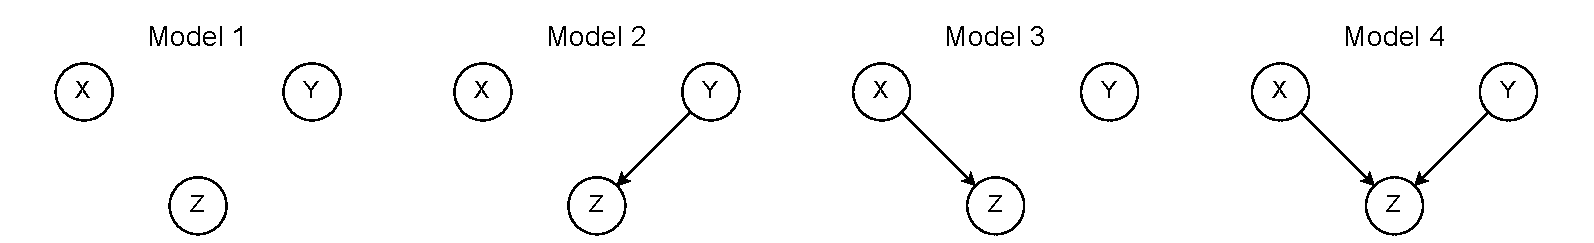
\includegraphics[width=0.95\textwidth]{pics/xyz_models.pdf}
    \caption{Models for \cref{example:model_selection}.}
    \label{fig:xyz_models}
\end{figure}



\subsection{Bayesian Linear Regression}

Let's consider the classical ML example --- linear regression.
The likelihood for linear regression is given as follows
\begin{align}
    p(y\cond x, \theta) = \Normal(y\cond w^Tx, \beta^{-1}) = \sqrt{\frac{\beta}{2\pi}}\exp\left(-\frac{\beta}{2}(y-w^Tx)^2\right)\,.
\end{align}
It's useful to think in terms of the log-likelihood, though, i.e.
\begin{align}
    \log p(y\cond x, \theta) = \log\Normal(y\cond w^Tx, \beta^{-1}) = -\frac{\beta}{2}(y- w^Tx)^2 + \frac{1}{2}\log \frac{\beta}{2\pi}\,.
\end{align}
First, let's find the maximum likelihood estimator $\theta_{\text{ML}} = \argmax_\theta \log p(\mathcal{D}\cond x, \theta)$ for the dataset $\mathcal{D} = \{(x_i,y_i)\}_{i=1}^N$.
That is, the derivative of the likelihood is
\begin{align}
    \nabla_w\sum_i\log\Normal(y_i\cond w^Tx_i, \beta^{-1}) = -\nabla_w\sum_i\frac{\beta}{2}(y_i- w^Tx_i)^2 = \beta\sum_i(y_i- w^Tx_i)x_i = 0\,,
\end{align}
where $x_i \in \mathbb{R}^d$ is a feature-vector of the $i$-th object.
It's convenient for us to introduce matrix $X$ such that $X_{ij}$ is the $j$-th coordinate of vector $x_i$ (of $i$-th object) and vector $y$ that consists of all the labels $y_i$.
Thus, we have
\begin{align}
    \sum_i y_iX_{ik} - \sum_i\sum_j w_{j} X_{ij} X_{ik} =~& 0\,, \;\forall\; k\,,\\
    X^Ty - X^TX w  =~& 0 \implies w_{\text{MLE}} = (X^TX)^{-1}X^Ty\,.
    \label{eq:linreg_mle}
\end{align}
Note that we got the classic formula for the linear regression.
Analogously, we have
\begin{align}
   \deriv{}{\beta}\left[\sum_i\log\Normal(y_i\cond w^Tx_i, \beta^{-1})\right] = -\sum_{i=1}^N\frac{1}{2}(y_i- w^Tx_i)^2 + \frac{N}{2\beta} = 0\\
   \frac{1}{\beta_{\text{MLE}}} = \frac{1}{N}\sum_{i=1}^N(y_i- w^Tx_i)^2 = \frac{1}{N}\norm{y-Xw}^2\,.
\end{align}

Now, let's introduce the prior distribution for the weights $w$.
That is, we assume that the weights are sampled (apriori) from the Normal distribution with the diagonal covariance matrix as follows
\begin{align}
    w \sim \Normal(w\cond 0,A^{-1})\,,\;\;\text{ where }\;\; 
    A = \begin{bmatrix}
        \alpha_1 & & 0\\
        & \ddots & \\
        0 & & \alpha_d
    \end{bmatrix}\,.
\end{align}
The posterior distribution for this model is defined as
\begin{align}
    p(\theta\cond \mathcal{D}) \propto \prod_{i=1}^N p(y_i\cond x_i,\theta) p(\theta) = \prod_{i=1}^N \Normal(y_i\cond w^Tx_i, \beta^{-1})\Normal(w\cond 0, A^{-1})\,.\\
    F(w) \coloneqq \prod_{i=1}^N \Normal(y_i\cond w^Tx_i, \beta^{-1})\Normal(w\cond 0, A^{-1})\,.
\end{align}
In this context, it is much easier to work with the logarithm of the density rather than with the density itself. Thus, we have
\begin{align}
    \log F(w) =~& \sum_{i=1}^N\log\Normal(y_i\cond w^Tx_i, \beta^{-1}) + \log\Normal(w\cond 0, A^{-1}) \\
    =~& -\sum_{i=1}^N\frac{\beta}{2}(y_i- w^Tx_i)^2 + \frac{N}{2}\log \frac{\beta}{2\pi} - \frac{1}{2}w^TAw + \frac{1}{2}\log \det(A) - \frac{d}{2}\log 2\pi\\
    =~& -\frac{\beta}{2}\norm{y-Xw}^2 + \frac{N}{2}\log \beta - \frac{1}{2}w^TAw + \frac{1}{2}\log \det(A) - \frac{d+N}{2}\log 2\pi\,.
\end{align}
Note that this a quadratic function, which means that the Taylor expansion of this function is going to contain only the first $3$ terms, i.e.
\begin{align}
    \log F(w) =~& \log F(w_{\text{MAP}}) + \inner{\nabla \log F(w_{\text{MAP}})}{w-w_{\text{MAP}}} + \\
    ~&+\frac{1}{2} (w - w_{\text{MAP}})^T \nabla^2_{ww} \log F(w_{\text{MAP}}) (w - w_{\text{MAP}}) + \underbrace{\deriv{^3}{w^3} + \ldots}_{=0}\,.
\end{align}
Note that we make the expansion at the point $w_{\text{MAP}}$ which is the Maximum A posteriori estimate, i.e.
\begin{align}
    w_{\text{MAP}} = \argmax_{w} \log F(w)\,.
\end{align}
Hence, $\nabla \log F(w_{\text{MAP}}) = 0$ is the necessary condition for being an optimum.
Thus, we have
\begin{align}
    \log F(w) =~& \log F(w_{\text{MAP}}) +\frac{1}{2} (w - w_{\text{MAP}})^T \nabla^2_{ww} \log F(w_{\text{MAP}}) (w - w_{\text{MAP}})\,.
\end{align}
Let's find $w_{\text{MAP}}$ first.
Clearly, we have
\begin{align}
    ~&\nabla_w \log F(w) = \beta X^T(y-Xw) - A w = 0\\
    ~&\beta X^Ty - \beta X^TX w - Aw  = 0 \implies w_{\text{MAP}} = \beta(\beta X^TX + A)^{-1}X^Ty = (X^TX + \beta^{-1}A)^{-1}X^Ty\,,
\end{align}
And the second derivative is
\begin{align}
    \nabla^2_{ww} \log F(w) = - \beta X^TX - A\,.
\end{align}

Remember that 
\begin{align}
    p(w\cond \mathcal{D}) \propto F(w) \implies \log p(w\cond \mathcal{D}) = \log F(w) + \text{const}\,,
\end{align}
where the constant can be defined from the normalization of the density (indeed, $p(w\cond \mathcal{D})$ has to be a valid density).
However, taking this integral is absolutely unnecessary since we already see that 
\begin{align}
    p(w\cond \mathcal{D}) \propto \exp\left( - \frac{1}{2} (w - w_{\text{MAP}})^T(\beta X^TX + A) (w - w_{\text{MAP}})\right)\,.
\end{align}
Thus, we have the following posterior distribution
\begin{align}
    p(w\cond \mathcal{D}) = \Normal\left(w\cond \underbrace{(X^TX + \beta^{-1}A)^{-1}X^Ty}_{w_{\text{MAP}}}, (\beta X^TX + A)^{-1}\right)\,.
\end{align}

Let's find the evidence
\begin{align}
    p(\mathcal{D}\cond \alpha,\beta) = \int dw\; p(\mathcal{D}\cond w,\beta)p(w\cond \alpha)\,.
\end{align}
Clearly, using the previously introduced notation, we have
\begin{align}
    p(\mathcal{D}\cond \alpha,\beta) =~& \int dw\; F(w) = F(w_{\text{MAP}})\int dw\; \exp\left[-\frac{1}{2} (w - w_{\text{MAP}})^T (\beta X^TX + A) (w - w_{\text{MAP}})\right]\\
    =~& F(w_{\text{MAP}}) \frac{(2\pi)^{d/2}}{\sqrt{\det(\beta X^TX + A)}}
\end{align}
Thus, we have to find $F(w_{\text{MAP}})$.
Let's do it
\begin{align}
    \log F(w_{\text{MAP}}) + \text{const} ~&= -\frac{\beta}{2}\norm{y-Xw_{\text{MAP}}}^2 - \frac{1}{2}w_{\text{MAP}}^TAw_{\text{MAP}}\\
    ~&= -\frac{\beta}{2}\left(y^Ty-2y^TXw_{\text{MAP}} + w_{\text{MAP}}^TX^TXw_{\text{MAP}} \right) - \frac{1}{2}w_{\text{MAP}}^TAw_{\text{MAP}}\\
    ~&= -\frac{\beta}{2}\left(y^Ty-2y^TXw_{\text{MAP}}\right) -\frac{1}{2} w_{\text{MAP}}^T\left(\beta X^TX + A\right)w_{\text{MAP}}\\
    ~&= -\frac{\beta}{2}\left(y^Ty-2\beta y^TX\left(\beta X^TX + A\right)^{-1} X^Ty\right) -\frac{\beta^2}{2} y^TX\left(\beta X^TX + A\right)^{-1} X^Ty\\
    ~&= -\frac{\beta}{2}y^T\left(I-\beta X\left(\beta X^TX + A\right)^{-1} X^T\right)y\\
    ~&= -\frac{\beta}{2}y^T\left(I- X\left(X^TX + \beta^{-1}A\right)^{-1} X^T\right)y
\end{align}
For the last expression, we need the Woodbury matrix identity
\begin{align}
    \left(A + UCV\right)^{-1} = A^{-1} - A^{-1}U\left(C^{-1} + VA^{-1}U\right)^{-1}VA^{-1}\,.
\end{align}
Thus, we have
\begin{align}
    \log F(w_{\text{MAP}}) = -\frac{\beta}{2}y^T\left(I + \beta^{-1}XA^{-1}X^T\right)^{-1}y + \frac{N}{2}\log \beta + \frac{1}{2}\log \det(A) - \frac{d+N}{2}\log 2\pi\,.
\end{align}
Finally, the evidence is
\begin{align}
    p(\mathcal{D}\cond \alpha,\beta) = \frac{(2\pi)^{d/2}\beta^{N/2}\sqrt{\det(A)}}{(2\pi)^{(d+N)/2}\sqrt{\det\left(\beta X^TX + A\right)}}\exp\left(-\frac{\beta}{2}y^T\left(I + \beta^{-1}XA^{-1}X^T\right)^{-1}y\right)\,,
\end{align}
for which, we can use
\begin{align}
    \det(A + UV) = \det(I + VA^{-1}U)\det(A)
\end{align}
and get
\begin{align}
    \beta^d\det\left(X^TX + \beta^{-1}A\right) = \beta^d\det(\beta^{-1}A)\det(I + \beta^{-1}XAX^T) = \det(A)\det(I + \beta^{-1}XAX^T)\,.
\end{align}
Thus, we have
\begin{align}
    p(\mathcal{D}\cond \alpha,\beta) = \frac{\beta^{N/2}}{(2\pi)^{N/2}\sqrt{\det(I + \beta^{-1}XAX^T)}}\exp\left(-\frac{\beta}{2}y^T\left(I + \beta^{-1}XA^{-1}X^T\right)^{-1}y\right)\,,
\end{align}
which we can then optimize as follows
\begin{align}
    \alpha^*,\beta^* = \argmax_{\alpha,\beta} p(\mathcal{D}\cond \alpha,\beta)\,.
\end{align}

To find the optimum of this function, it is easier to consider the variational bound of this function
\begin{mybox}
    \begin{definition}[Variational Bound]\label{def:var_bound}
    We call the function $g(x,\xi)$ a variational bound of function $f(x)$ if
    \begin{enumerate}
        \item $\forall \; x,\xi\;\; f(x) \geq g(x,\xi)\,,$
        \item $\forall \; x\; \exists\; \xi_x \; : f(x) = g(x,\xi_x)\,.$
    \end{enumerate}
    \end{definition}
\end{mybox}

\begin{align}
    \log p(\mathcal{D}\cond \alpha,\beta) =~& -\frac{\beta}{2}\norm{y-Xw_{\text{MAP}}}^2 - \frac{1}{2}w_{\text{MAP}}^TAw_{\text{MAP}} + \\
    ~&+ \frac{N}{2}\log \beta + \frac{1}{2}\log \det(A) - \frac{N}{2}\log 2\pi - \frac{1}{2}\log \det(\beta X^TX + A)\\
    \geq~& -\frac{\beta}{2}\norm{y-Xw}^2 - \frac{1}{2}w^TAw + \\
    ~&+ \frac{N}{2}\log \beta + \frac{1}{2}\log \det(A) - \frac{N}{2}\log 2\pi - \frac{1}{2}\log \det(\beta X^TX + A) \coloneqq \hat{F}(w,\alpha,\beta)
\end{align}

\begin{align}
    \deriv{}{w}\hat{F}(w,\alpha,\beta) = -\beta X^T(y - Xw) = 0 \implies w = w_{\text{MAP}}\,.
\end{align}

\begin{align}
    \deriv{}{\alpha_j}\hat{F}(w,\alpha,\beta) =~& -\frac{1}{2}w^2_j + \frac{1}{2}\frac{1}{\alpha_j} - \frac{1}{2} \inner{(\beta X^TX + A)^{-1}}{\deriv{}{\alpha_j}(\beta X^TX + A)} \\
    =~& -\frac{1}{2}w^2_j+ \frac{1}{2}\frac{1}{\alpha_j} - \frac{1}{2} (\beta X^TX + A)^{-1}_{jj} = 0\\
    \alpha_j =~& \frac{1}{w_j^2 + (\beta X^TX + A)^{-1}_{jj}}
\end{align}

\begin{align}
    \deriv{}{\beta}\hat{F}(w,\alpha,\beta) =~& -\frac{1}{2}\norm{y - Xw}^2 + \frac{N}{2\beta} - \frac{1}{2}\inner{(\beta X^TX + A)^{-1}}{\deriv{}{\beta}(\beta X^TX + A)}\\
    =~& -\frac{1}{2}\norm{y - Xw}^2 + \frac{N}{2\beta} - \frac{1}{2\beta}\inner{(\beta X^TX + A)^{-1}}{\beta X^TX \pm A}\\
    =~& -\frac{1}{2}\norm{y - Xw}^2 + \frac{N}{2\beta} - \frac{1}{2\beta}(d - \sum_j\alpha_j (\beta X^TX + A)^{-1}_{jj}) = 0\\
    \beta =~& \frac{N - d + \sum_j\alpha_j (\beta X^TX + A)^{-1}_{jj}}{\norm{y - Xw}^2}
\end{align}

\begin{exercise}
    Find the predictive distribution, i.e.
    \begin{align}
        p(y\cond x,\alpha,\beta)= \int dw\; \Normal(y\cond w^Tx, \beta^{-1})p(w\cond \mathcal{D}) = ?
    \end{align}
\end{exercise}

\subsection{Bayesian Logistic Regression, Laplace Approximation}

Consider the Logistic Regression for classification problem $y \in \{-1,1\}$
\begin{align}
    p(y\cond x,w) = \frac{1}{1+\exp(-yw^Tx)}
\end{align}
With the normal prior
\begin{align}
    p(w) = \Normal(w\cond 0, A^{-1})\,,\;\;\text{ where }\;\; 
    A = \begin{bmatrix}
        \alpha_1 & & 0\\
        & \ddots & \\
        0 & & \alpha_d
    \end{bmatrix}\,.
\end{align}

The posterior distribution is
\begin{align}
    p(w\cond \mathcal{D}) \propto \prod_i p(y_i\cond x_i,w) \Normal(w\cond 0, A^{-1})
\end{align}
\begin{align}
    \log p(w\cond \mathcal{D}) + \log Z =~& \sum_i \log p(y_i \cond x_i, w) - \frac{1}{2}w^TAw + \frac{1}{2} \log \det (A) - \frac{d}{2}\log (2\pi) \\
    =~& -\sum_i \log (1+\exp(-y_iw^Tx_i)) - \frac{1}{2}w^TAw + \frac{1}{2} \log \det (A) - \frac{d}{2}\log (2\pi) \coloneqq \log F(w)\,.
\end{align}
Let's do the same expansion as we did for the linear regression
\begin{align}
    \log F(w) =~& \log F(w_{\text{MAP}}) + \inner{\nabla \log F(w_{\text{MAP}})}{w-w_{\text{MAP}}} + \\
    ~&+\frac{1}{2} (w - w_{\text{MAP}})^T \deriv{^2}{w^2} \log F(w_{\text{MAP}}) (w - w_{\text{MAP}}) + \underbrace{\deriv{^3}{w^3} + \ldots}_{\neq 0}\,.
\end{align}
The last terms are not zero anymore, but this is an approximation.
Even for this, it's not trivial to find $w_{\text{MAP}}$
\begin{align}
    \nabla_w \log F(w) =~& -\sum_i \frac{\exp(-y_iw^Tx_i)}{1+\exp(-y_iw^Tx_i)}(-y_ix_i) - Aw = \sum_i \frac{1}{1+\exp(y_iw^Tx_i)}y_ix_i - Aw\\
    \deriv{^2}{w^2} \log F(w) =~& -\sum_i \frac{\exp(y_iw^Tx_i)}{(1+\exp(y_iw^Tx_i))^2}x_i x_i^T - A = -X^TR(w)X - A\,,
\end{align}
where $R(w)$ is the diagonal matrix with the elements
\begin{align}
    R(w)_{ii} = \frac{\exp(y_iw^Tx_i)}{(1+\exp(y_iw^Tx_i))^2}\,.
\end{align}
Thus, we approximate the posterior distribution as follows 
\begin{align}
    p(w\cond D) \propto F(w) \propto \Normal(w\cond w_{\text{MAP}}, (X^TR(w_{\text{MAP}})X + A)^{-1})\,.
\end{align}
Of course, this approximation is not specific to the logistic regression but a general technique that can be summarized as follows.
\begin{mybox}
\begin{definition}[Laplace approximation]
\label{def:laplace}
    For a given density $p(x)$ the Laplace approximation is 
    \begin{align}
        p(x) \approx \Normal(x\cond \mu, \Sigma)\,,\; \mu = \argmax_x p(x)\,,\;\; \Sigma^{-1} = -\nabla^2_{xx}\log p(x)\,.
    \end{align}
\end{definition}    
\end{mybox}


\begin{align}
    p(\mathcal{D}\cond A) = \int dw\; \prod_i p(y_i\cond x_i,w) \Normal(w\cond 0, A^{-1})
\end{align}
